\section{Results}
\label{sec:results}

Table~\ref{tab:loglikelihood} summarizes the results of the
experiments comparing the eight combinations over the different
scenarios. The empirical hybridization is denoted as \emph{EMP}, and
the reduced representation as \emph{Red}.

\begin{table}
  \caption{Log Likelihood Values for each scenario and
    combination. Higher values correspond to better models. Values in
    bold are the two highest log likelihood for a scenario. Each value
    is the average of 10 runs.}
  \label{tab:loglikelihood}
  \begin{tabular}{|c|c|c|c|c|c|c|c|c|}
    \hline
    & \multicolumn{4}{|c|}{No Pre-processing} & \multicolumn{4}{|c|}{Spectral Clustering}\\
    Scenario & GA & Red & EMP & EMP-Red & GA & Red & EMP & EMP-Red\\
    \hline
    Kanto 2005 & -2291.4 & -2354.1 & -2345.1 & -2557.8 & {\bf-2202.7} & -2233.3 & {\bf-2203.7} & -2355.0\\
    Kanto 2006 & -2269.2 & -2317.3 & -2350.7 & -2520.0 & {\bf-2173.3} & -2203.1 & {\bf-2175.8} & -2313.5\\
    Kanto 2007 & -2204.9 & -2235.7 & -2293.3 & -2449.5 & {\bf-2104.1} & -2125.0 & {\bf-2110.3} & -2213.9\\
    Kanto 2008 & -2203.0 & -2273.2 & -2277.7 & -2501.0 & {\bf-2097.9} & -2124.3 & {\bf-2010.3} & -2245.7\\
    Kanto 2009 & -2375.6 & -2418.5 & -2463.6 & -2630.7 & {\bf-2279.1} & -2299.1 & {\bf-2282.4} & -2382.0\\
    Kanto 2010 & -2203.6 & -2296.6 & -2294.9 & -2534.4 & {\bf-2099.5} & -2125.0 & {\bf-2104.0} & -2249.8\\
    \hline
    EastJapan 2005 &-2442.8&-2394.9&-2633.6&-2588.4& {\bf-2099.6} & {\bf-2150.2} & -2177.4 & -2300.6 \\
    EastJapan 2006 &-2211.1&-2191.7&-2408.9&-2390.9&{\bf-1896.7}&{\bf-1960.4}&-1965.7&-2131.8\\
    EastJapan 2007 &-2112.2&-2100.5&-2305.1&-2294.9&{\bf-1821.9}&{\bf-1889.4}&-1914.4&-2070.0\\
    EastJapan 2008 &-4139.7&-4288.6&-4301.3&-4424.8&{\bf-3942.5}&{\bf-3989.1}&-4034.9&-4156.8\\
    EastJapan 2009 &-2281.2&-2221.2&-2498.9&-2416.5&{\bf-1948.5}&{\bf-1087.4}&-2043.7&-2164.5\\
    EastJapan 2010 &-2577.7&-2579.1&-2783.9&-2783.9&{\bf-2232.7}&{\bf-2291.3}&-2296.9&-2455.2\\
    \hline
  \end{tabular}
\end{table}

%% ANOVA ANALYSIS

To better understand these results, we perform an ANOVA analysis...

* Anova in all areas

Because the anova indicated a significant difference, we use Tukey's
HSD to see which combination showed this difference ...

* HSD Tukey against GAModel

%% HEAT MAP

To get a better intuition about what these results mean in concrete
terms, we show a selection of the actual models... (explain heat map)

\begin{figure}
\centering
\begin{subfigure}{.5\textwidth}
  \centering
  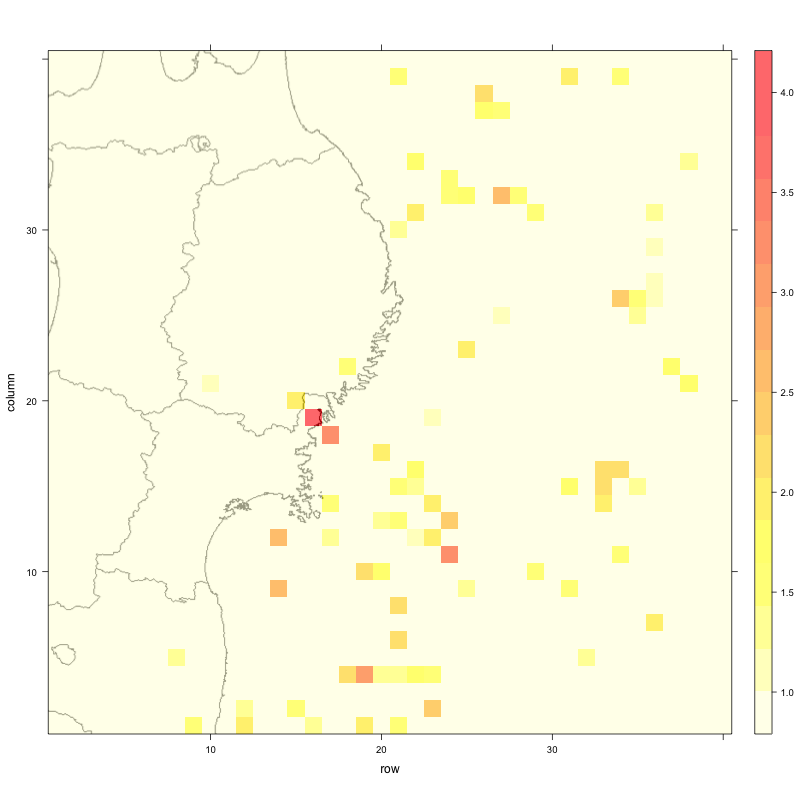
\includegraphics[width=1\linewidth]{img/gaModel}
  \caption{GAModel}
  \label{fig:sub1}
\end{subfigure}%
\begin{subfigure}{.5\textwidth}
  \centering
  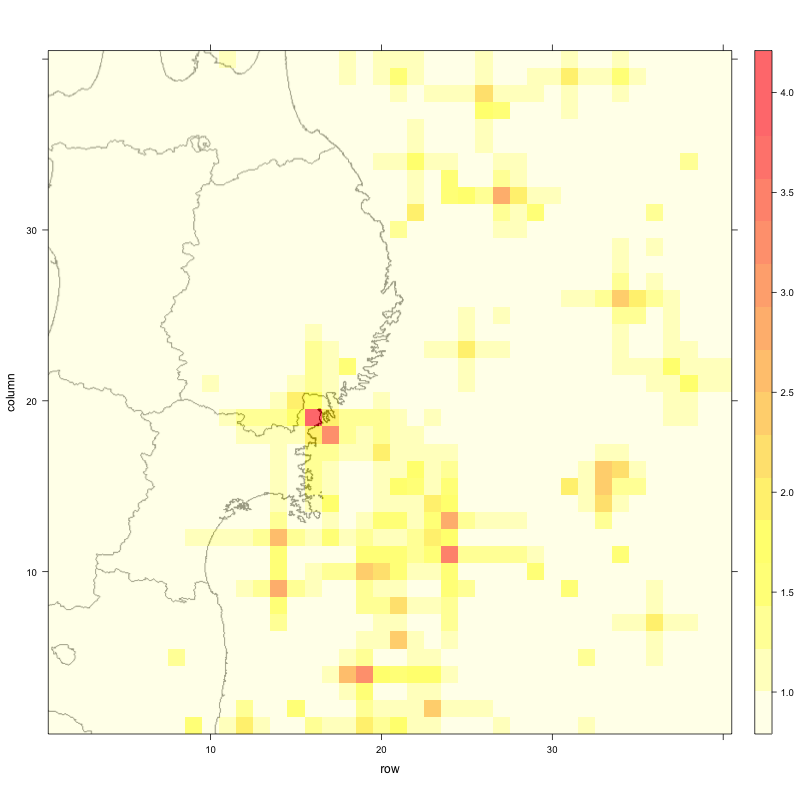
\includegraphics[width=1\linewidth]{img/SC-EMP-ga}
  \caption{Spectral Clustering with Emp-GA}
  \label{fig:sub2}
\end{subfigure}\\
\begin{subfigure}{.5\textwidth}
  \centering
  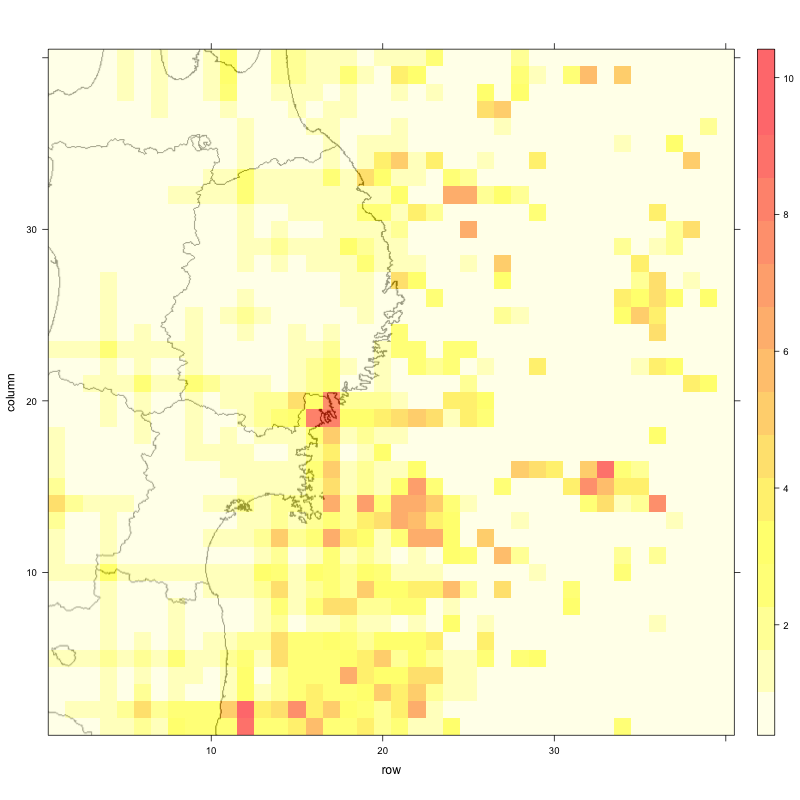
\includegraphics[width=1\linewidth]{img/EMP-RED-ga}
  \caption{EMP-GA with Reduced Representation}
  \label{fig:sub3}
\end{subfigure}%
\begin{subfigure}{.5\textwidth}
  \centering
  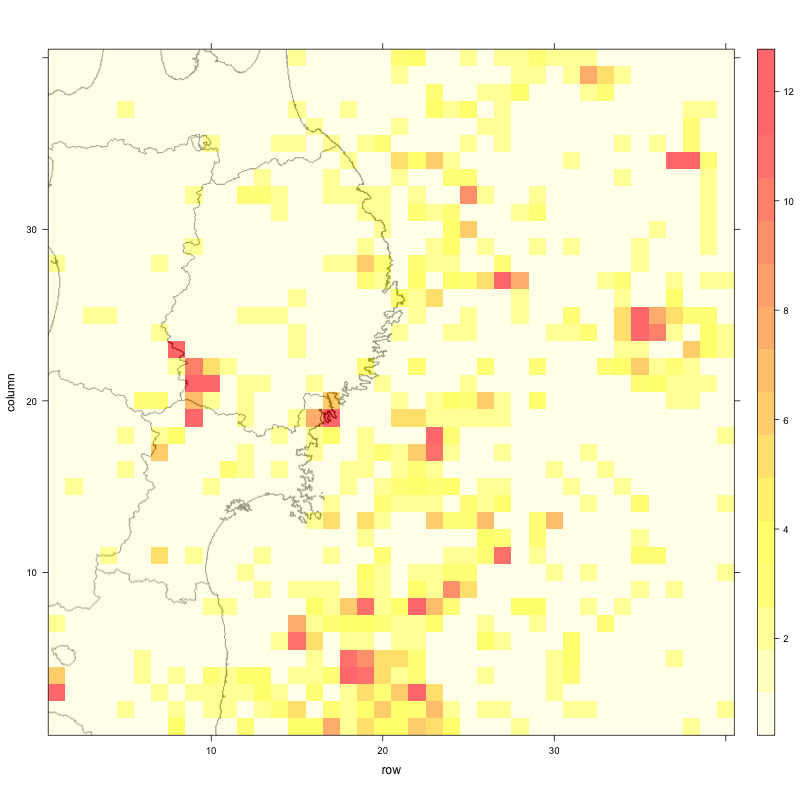
\includegraphics[width=1\linewidth]{img/realEastJapan_2010}
  \caption{Earthquake Catalog}
  \label{fig:sub4}
\end{subfigure}
\caption{Earthquake Risk Model Heatmaps, for scenario East Japan
  2010. Darker colors correspond to higher number of earthquakes}
\label{fig:test}
\end{figure}

